\documentclass[11pt,a4paper,oneside]{report}
\usepackage[utf8]{inputenc}
\usepackage[T1]{fontenc}
\usepackage[english]{babel}
\usepackage{lmodern}
\usepackage{microtype}
\usepackage[a4paper,margin=1.80cm]{geometry}
\usepackage{amsmath}
\usepackage{amssymb}
\usepackage{graphicx}
\usepackage{booktabs}
\usepackage{array}
\usepackage{tabularx}
\usepackage{caption}
\usepackage{xcolor}
\usepackage{etoolbox}

\usepackage{tikz}
\usetikzlibrary{shapes.geometric,arrows.meta,positioning,calc}
\usepackage{acro}
% Acronyms declared for the thesis
% Loaded in main.tex via % Acronyms declared for the thesis
% Loaded in main.tex via % Acronyms declared for the thesis
% Loaded in main.tex via \input{acronyms}
% Use \ac{label} in text: expands on first use, short form thereafter.

\DeclareAcronym{api}{
  short = API,
  long  = Application Programming Interface
}
\DeclareAcronym{cps2}{
  short = CPS2,
  long  = Cyber Physical and Social Systems
}
\DeclareAcronym{bsd}{
  short = BSD,
  long  = Berkeley Software Distribution
}
\DeclareAcronym{cdt}{
  short = CDT,
  long  = Custom Datatypes
}
\DeclareAcronym{dicom}{
  short = DICOM,
  long  = Digital Imaging and Communications in Medicine
}
\DeclareAcronym{fhir}{
  short = FHIR,
  long  = Fast Healthcare Interoperability Resources
}
\DeclareAcronym{gml}{
  short = GML,
  long  = Geography Markup Language
}
\DeclareAcronym{hl7}{
  short = HL7,
  long  = Health Level Seven
}
\DeclareAcronym{http}{
  short = HTTP,
  long  = Hypertext Transfer Protocol
}
\DeclareAcronym{iri}{
  short = IRI,
  long  = Internationalized Resource Identifier
}
\DeclareAcronym{iso}{
  short = ISO,
  long  = International Organization for Standardization
}
\DeclareAcronym{jcgm}{
  short = JCGM,
  long  = Joint Committee for Guides in Metrology
}
\DeclareAcronym{json}{
  short = JSON,
  long  = JavaScript Object Notation
}
\DeclareAcronym{jsonld}{
  short = JSON-LD,
  long  = JSON for Linking Data
}
\DeclareAcronym{jsr}{
  short = JSR,
  long  = Java Specification Request
}
\DeclareAcronym{lindt}{
  short = LINDT,
  long  = Linked Datatypes
}
\DeclareAcronym{loinc}{
  short = LOINC,
  long  = Logical Observation Identifiers Names and Codes
}
\DeclareAcronym{muo}{
  short = MUO,
  long  = Measurement Units Ontology
}
\DeclareAcronym{nasa}{
  short = NASA,
  long  = National Aeronautics and Space Administration
}
\DeclareAcronym{oboe}{
  short = OBOE,
  long  = Extensible Observation Ontology
}
\DeclareAcronym{ogc}{
  short = OGC,
  long  = Open Geospatial Consortium
}
\DeclareAcronym{om}{
  short = OM,
  long  = Ontology of units of Measure
}
\DeclareAcronym{owl}{
  short = OWL,
  long  = Web Ontology Language
}
\DeclareAcronym{qu}{
  short = QU,
  long  = Quantities and Units
}
\DeclareAcronym{qudt}{
  short = QUDT,
  long  = {Quantities, Units, Dimensions and Data Types Ontologies}
}
\DeclareAcronym{rdf}{
  short = RDF,
  long  = Resource Description Framework
}
\DeclareAcronym{rdfa}{
  short = RDFa,
  long  = RDF in Attributes
}
\DeclareAcronym{rdfs}{
  short = RDFS,
  long  = RDF Schema
}
\DeclareAcronym{rfc}{
  short = RFC,
  long  = Request for Comments
}
\DeclareAcronym{shacl}{
  short = SHACL,
  long  = Shapes Constraint Language
}
\DeclareAcronym{si}{
  short = SI,
  long  = International System of Units
}
\DeclareAcronym{sosa}{
  short = SOSA,
  long  = {Sensor, Observation, Sample, and Actuator}
}
\DeclareAcronym{sparql}{
  short = SPARQL,
  long  = SPARQL Protocol and RDF Query Language
}
\DeclareAcronym{ssn}{
  short = SSN,
  long  = Semantic Sensor Network
}
\DeclareAcronym{sweet}{
  short = SWEET,
  long  = Semantic Web for Earth and Environmental Terminology
}
\DeclareAcronym{ucum}{
  short = UCUM,
  long  = Unified Code for Units of Measure
}
\DeclareAcronym{uo}{
  short = UO,
  long  = Units Ontology
}
\DeclareAcronym{vim}{
  short = VIM,
  long  = International Vocabulary of Metrology
}
\DeclareAcronym{w3c}{
  short = W3C,
  long  = World Wide Web Consortium
}
\DeclareAcronym{webdav}{
  short = WebDAV,
  long  = Web Distributed Authoring and Versioning
}
\DeclareAcronym{wkt}{
  short = WKT,
  long  = Well-Known Text
}
\DeclareAcronym{xml}{
  short = XML,
  long  = Extensible Markup Language
}
\DeclareAcronym{xsd}{
  short = XSD,
  long  = XML Schema Definition
}
\DeclareAcronym{omg}{
  short = OMG,
  long  = Object Management Group
}
\DeclareAcronym{obo}{
  short = OBO,
  long  = Open Biological and Biomedical Ontologies
}
\DeclareAcronym{pato}{
  short = PATO,
  long  = Phenotypic Quality Ontology
}
\DeclareAcronym{qudv}{
  short = QUDV,
  long  = {Quantities, Units, Dimensions and Values}
}
\DeclareAcronym{uncefact}{
  short = UN/CEFACT,
  long  = {United Nations Centre for Trade Facilitation and Electronic Business}
}

\DeclareAcronym{us}{
short = US, 
long = United States
}

% Use \ac{label} in text: expands on first use, short form thereafter.

\DeclareAcronym{api}{
  short = API,
  long  = Application Programming Interface
}
\DeclareAcronym{cps2}{
  short = CPS2,
  long  = Cyber Physical and Social Systems
}
\DeclareAcronym{bsd}{
  short = BSD,
  long  = Berkeley Software Distribution
}
\DeclareAcronym{cdt}{
  short = CDT,
  long  = Custom Datatypes
}
\DeclareAcronym{dicom}{
  short = DICOM,
  long  = Digital Imaging and Communications in Medicine
}
\DeclareAcronym{fhir}{
  short = FHIR,
  long  = Fast Healthcare Interoperability Resources
}
\DeclareAcronym{gml}{
  short = GML,
  long  = Geography Markup Language
}
\DeclareAcronym{hl7}{
  short = HL7,
  long  = Health Level Seven
}
\DeclareAcronym{http}{
  short = HTTP,
  long  = Hypertext Transfer Protocol
}
\DeclareAcronym{iri}{
  short = IRI,
  long  = Internationalized Resource Identifier
}
\DeclareAcronym{iso}{
  short = ISO,
  long  = International Organization for Standardization
}
\DeclareAcronym{jcgm}{
  short = JCGM,
  long  = Joint Committee for Guides in Metrology
}
\DeclareAcronym{json}{
  short = JSON,
  long  = JavaScript Object Notation
}
\DeclareAcronym{jsonld}{
  short = JSON-LD,
  long  = JSON for Linking Data
}
\DeclareAcronym{jsr}{
  short = JSR,
  long  = Java Specification Request
}
\DeclareAcronym{lindt}{
  short = LINDT,
  long  = Linked Datatypes
}
\DeclareAcronym{loinc}{
  short = LOINC,
  long  = Logical Observation Identifiers Names and Codes
}
\DeclareAcronym{muo}{
  short = MUO,
  long  = Measurement Units Ontology
}
\DeclareAcronym{nasa}{
  short = NASA,
  long  = National Aeronautics and Space Administration
}
\DeclareAcronym{oboe}{
  short = OBOE,
  long  = Extensible Observation Ontology
}
\DeclareAcronym{ogc}{
  short = OGC,
  long  = Open Geospatial Consortium
}
\DeclareAcronym{om}{
  short = OM,
  long  = Ontology of units of Measure
}
\DeclareAcronym{owl}{
  short = OWL,
  long  = Web Ontology Language
}
\DeclareAcronym{qu}{
  short = QU,
  long  = Quantities and Units
}
\DeclareAcronym{qudt}{
  short = QUDT,
  long  = {Quantities, Units, Dimensions and Data Types Ontologies}
}
\DeclareAcronym{rdf}{
  short = RDF,
  long  = Resource Description Framework
}
\DeclareAcronym{rdfa}{
  short = RDFa,
  long  = RDF in Attributes
}
\DeclareAcronym{rdfs}{
  short = RDFS,
  long  = RDF Schema
}
\DeclareAcronym{rfc}{
  short = RFC,
  long  = Request for Comments
}
\DeclareAcronym{shacl}{
  short = SHACL,
  long  = Shapes Constraint Language
}
\DeclareAcronym{si}{
  short = SI,
  long  = International System of Units
}
\DeclareAcronym{sosa}{
  short = SOSA,
  long  = {Sensor, Observation, Sample, and Actuator}
}
\DeclareAcronym{sparql}{
  short = SPARQL,
  long  = SPARQL Protocol and RDF Query Language
}
\DeclareAcronym{ssn}{
  short = SSN,
  long  = Semantic Sensor Network
}
\DeclareAcronym{sweet}{
  short = SWEET,
  long  = Semantic Web for Earth and Environmental Terminology
}
\DeclareAcronym{ucum}{
  short = UCUM,
  long  = Unified Code for Units of Measure
}
\DeclareAcronym{uo}{
  short = UO,
  long  = Units Ontology
}
\DeclareAcronym{vim}{
  short = VIM,
  long  = International Vocabulary of Metrology
}
\DeclareAcronym{w3c}{
  short = W3C,
  long  = World Wide Web Consortium
}
\DeclareAcronym{webdav}{
  short = WebDAV,
  long  = Web Distributed Authoring and Versioning
}
\DeclareAcronym{wkt}{
  short = WKT,
  long  = Well-Known Text
}
\DeclareAcronym{xml}{
  short = XML,
  long  = Extensible Markup Language
}
\DeclareAcronym{xsd}{
  short = XSD,
  long  = XML Schema Definition
}
\DeclareAcronym{omg}{
  short = OMG,
  long  = Object Management Group
}
\DeclareAcronym{obo}{
  short = OBO,
  long  = Open Biological and Biomedical Ontologies
}
\DeclareAcronym{pato}{
  short = PATO,
  long  = Phenotypic Quality Ontology
}
\DeclareAcronym{qudv}{
  short = QUDV,
  long  = {Quantities, Units, Dimensions and Values}
}
\DeclareAcronym{uncefact}{
  short = UN/CEFACT,
  long  = {United Nations Centre for Trade Facilitation and Electronic Business}
}

\DeclareAcronym{us}{
short = US, 
long = United States
}

% Use \ac{label} in text: expands on first use, short form thereafter.

\DeclareAcronym{api}{
  short = API,
  long  = Application Programming Interface
}
\DeclareAcronym{cps2}{
  short = CPS2,
  long  = Cyber Physical and Social Systems
}
\DeclareAcronym{bsd}{
  short = BSD,
  long  = Berkeley Software Distribution
}
\DeclareAcronym{cdt}{
  short = CDT,
  long  = Custom Datatypes
}
\DeclareAcronym{dicom}{
  short = DICOM,
  long  = Digital Imaging and Communications in Medicine
}
\DeclareAcronym{fhir}{
  short = FHIR,
  long  = Fast Healthcare Interoperability Resources
}
\DeclareAcronym{gml}{
  short = GML,
  long  = Geography Markup Language
}
\DeclareAcronym{hl7}{
  short = HL7,
  long  = Health Level Seven
}
\DeclareAcronym{http}{
  short = HTTP,
  long  = Hypertext Transfer Protocol
}
\DeclareAcronym{iri}{
  short = IRI,
  long  = Internationalized Resource Identifier
}
\DeclareAcronym{iso}{
  short = ISO,
  long  = International Organization for Standardization
}
\DeclareAcronym{jcgm}{
  short = JCGM,
  long  = Joint Committee for Guides in Metrology
}
\DeclareAcronym{json}{
  short = JSON,
  long  = JavaScript Object Notation
}
\DeclareAcronym{jsonld}{
  short = JSON-LD,
  long  = JSON for Linking Data
}
\DeclareAcronym{jsr}{
  short = JSR,
  long  = Java Specification Request
}
\DeclareAcronym{lindt}{
  short = LINDT,
  long  = Linked Datatypes
}
\DeclareAcronym{loinc}{
  short = LOINC,
  long  = Logical Observation Identifiers Names and Codes
}
\DeclareAcronym{muo}{
  short = MUO,
  long  = Measurement Units Ontology
}
\DeclareAcronym{nasa}{
  short = NASA,
  long  = National Aeronautics and Space Administration
}
\DeclareAcronym{oboe}{
  short = OBOE,
  long  = Extensible Observation Ontology
}
\DeclareAcronym{ogc}{
  short = OGC,
  long  = Open Geospatial Consortium
}
\DeclareAcronym{om}{
  short = OM,
  long  = Ontology of units of Measure
}
\DeclareAcronym{owl}{
  short = OWL,
  long  = Web Ontology Language
}
\DeclareAcronym{qu}{
  short = QU,
  long  = Quantities and Units
}
\DeclareAcronym{qudt}{
  short = QUDT,
  long  = {Quantities, Units, Dimensions and Data Types Ontologies}
}
\DeclareAcronym{rdf}{
  short = RDF,
  long  = Resource Description Framework
}
\DeclareAcronym{rdfa}{
  short = RDFa,
  long  = RDF in Attributes
}
\DeclareAcronym{rdfs}{
  short = RDFS,
  long  = RDF Schema
}
\DeclareAcronym{rfc}{
  short = RFC,
  long  = Request for Comments
}
\DeclareAcronym{shacl}{
  short = SHACL,
  long  = Shapes Constraint Language
}
\DeclareAcronym{si}{
  short = SI,
  long  = International System of Units
}
\DeclareAcronym{sosa}{
  short = SOSA,
  long  = {Sensor, Observation, Sample, and Actuator}
}
\DeclareAcronym{sparql}{
  short = SPARQL,
  long  = SPARQL Protocol and RDF Query Language
}
\DeclareAcronym{ssn}{
  short = SSN,
  long  = Semantic Sensor Network
}
\DeclareAcronym{sweet}{
  short = SWEET,
  long  = Semantic Web for Earth and Environmental Terminology
}
\DeclareAcronym{ucum}{
  short = UCUM,
  long  = Unified Code for Units of Measure
}
\DeclareAcronym{uo}{
  short = UO,
  long  = Units Ontology
}
\DeclareAcronym{vim}{
  short = VIM,
  long  = International Vocabulary of Metrology
}
\DeclareAcronym{w3c}{
  short = W3C,
  long  = World Wide Web Consortium
}
\DeclareAcronym{webdav}{
  short = WebDAV,
  long  = Web Distributed Authoring and Versioning
}
\DeclareAcronym{wkt}{
  short = WKT,
  long  = Well-Known Text
}
\DeclareAcronym{xml}{
  short = XML,
  long  = Extensible Markup Language
}
\DeclareAcronym{xsd}{
  short = XSD,
  long  = XML Schema Definition
}
\DeclareAcronym{omg}{
  short = OMG,
  long  = Object Management Group
}
\DeclareAcronym{obo}{
  short = OBO,
  long  = Open Biological and Biomedical Ontologies
}
\DeclareAcronym{pato}{
  short = PATO,
  long  = Phenotypic Quality Ontology
}
\DeclareAcronym{qudv}{
  short = QUDV,
  long  = {Quantities, Units, Dimensions and Values}
}
\DeclareAcronym{uncefact}{
  short = UN/CEFACT,
  long  = {United Nations Centre for Trade Facilitation and Electronic Business}
}

\DeclareAcronym{us}{
short = US, 
long = United States
}

\usepackage{titlesec}
\makeatletter
\renewcommand{\thetable}{\arabic{table}}
\@removefromreset{table}{chapter}
% Remove forced new page before each chapter
\patchcmd{\chapter}{\if@openright\cleardoublepage\else\clearpage\fi}{\par\vspace{2em}}{}{}
\makeatother
% Chapter heading: numbered, reduced to \LARGE (was \Huge)
\titleformat{\chapter}[hang]{\normalfont\LARGE\bfseries}{\thechapter.}{0.5em}{}
\titlespacing*{\chapter}{0pt}{3em}{1em}
\usepackage[backend=biber,style=numeric]{biblatex}
\addbibresource{references.bib}
\DeclareSortingTemplate{original}{
  \sort{\field{sortkey}}
}
\ExecuteBibliographyOptions{sorting=original}
\usepackage[colorlinks=true,linkcolor=black,citecolor=black,urlcolor=blue]{hyperref}
\begin{document}
\pagenumbering{roman}
\begin{titlepage}
  % Logos
  \noindent
  \begin{minipage}[t]{0.4\textwidth}
    \raggedright
    
\includegraphics[height=2.5cm]{Logo_de_l'Université_Jean_Monnet_Saint-Etienne.png}
  \end{minipage}%
  \hfill%
  \begin{minipage}[t]{0.4\textwidth}
    \raggedleft
    
\includegraphics[height=2.3cm]{images.png}
  \end{minipage}
  \par\vspace{1cm}
  \centering
  %% - DEGREE SIDE  -
  {\large Université de Lyon\par}
  \vspace{0.25cm}
  {\normalsize
    Université Jean Monnet Saint-Étienne
\textperiodcentered\
    Mines Saint-Étienne - Institut Mines Télécom\par
  }
  \vspace{0.2cm}
  {\small Master in Computer Science -
    Cyber-Physical and Social Systems: AI and IoT (CPS2)\par}
  \vspace{0.6cm}
  \hrule
  \vspace{0.8cm}
  %% - TITLE  --
  {\Huge\bfseries Representation of Physical Quantities\\[0.3em]
    on the Semantic Web\par}
  \vspace{0.8cm}
  {\normalsize
    M2 Internship Thesis submitted in partial fulfillment\\
    of the requirements for the degree of\\[0.2em]
    \textbf{Master 2 in Computer Science}\par
  }
  \vspace{1cm}
  %% - STUDENT  --
  {\large Irfan Ullah\par}
  \vspace{0.2cm}
  {\small Academic year 2024-2026\par}
  \vspace{1cm}
  \hrule
  \vspace{0.8cm}
  %% - INTERNSHIP SIDE  ---
  {\small Mandatory research internship conducted at\par}
  \vspace{0.2cm}
  {\normalsize\bfseries
    Département Informatique et Systèmes Intelligents (ISI)\\
    Institut Henri Fayol - Mines Saint-Étienne\par}
  \vspace{0.15cm}

  \vspace{0.15cm}
  {\small 1 February 2026 - 30 June 2026\par}
  \vspace{0.6cm}
{\small Supervised by\par}
\vspace{0.4cm}
\noindent
\begin{minipage}[t]{0.47\textwidth}
  \centering
  {\normalsize\textbf{Antoine Zimmermann}\par}
  \vspace{0.1cm}
  {\small Professor\par}
  {\small Head of ISI Department\par}
  {\small Institut Henri Fayol\par}
  {\small École des Mines de Saint-Étienne\par}
  {\small LIMOS - UMR CNRS 6158\par}
  \vspace{0.1cm}
  {\small \href{mailto:antoine.zimmermann@emse.fr}{antoine.zimmermann@emse.fr}\par}
\end{minipage}%
\hfill%
\begin{minipage}[t]{0.47\textwidth}
  \centering
  {\normalsize\textbf{Maxime Lefrançois}\par}
  \vspace{0.1cm}
  {\small Associate Professor\par}
  {\small Institut Henri Fayol\par}
  {\small École des Mines de Saint-Étienne\par}
  {\small LIMOS - UMR CNRS 6158\par}
  \vspace{0.1cm}
  {\small \href{mailto:maxime.lefrancois@emse.fr}{maxime.lefrancois@emse.fr}\par}
\end{minipage}
  \vfill
  {\normalsize \today\par}
\end{titlepage}
\clearpage
\chapter*{Abstract}
\addcontentsline{toc}{chapter}{Abstract}

Physical quantities are fundamental to scientific, engineering, and medical data on the Semantic Web. The dominant approach is ontology-based: \ac{qudt} and \ac{om} provide quantity kinds, unit hierarchies, dimensional vectors, and conversion factors. But four problems persist regardless of ontological richness. The most serious is computational inaccessibility: dimensional structure is encoded in the graph but never reaches the \ac{sparql} expression evaluator, so comparisons, ordering, and aggregation over mixed-unit data produce physically incomplete results without warning. The second is bounded coverage: derived units multiply combinatorial and no enumeration can be complete. The third is interoperability: independently developed ontologies assign different \acp{iri} to the same physical unit, requiring manual cross-ontology mappings. The fourth is verbosity: a single quantity value requires at least three triples.

The \ac{lindt} specification addresses all four problems at the datatype level through \texttt{cdt:ucum}, which encodes a complete quantity as a single typed literal using \ac{ucum}. Because \ac{ucum} is a grammar rather than a list, coverage is unlimited by construction. The value space recognises dimensional equivalence natively, and operator semantics expose unit-aware equality, comparison, and arithmetic directly within \ac{sparql}. The only existing implementation is a fork of Apache Jena and it is outdated, and no implementation exists for any other major \ac{rdf} library. No general, reproducible procedure for building one has been documented.

This thesis addresses that gap. It presents a five-step methodology covering candidate library identification, extension point analysis, feasibility assessment, implementation, and validation. The feasibility step is an explicit go/no-go decision point before any code is written, and its output records not only whether each obligation can be met but through what mechanism and at what stability cost. A hard constraint frames the assessment: the implementation must leave the host library unmodified.

The methodology is validated through four working implementations across Apache Jena in Java, rdflib.js in TypeScript, dotNetRDF in C\#, and RDFLib in Python, each paired with a \ac{ucum} backend suited to its ecosystem and accompanied by a test suite written against a single shared reference checklist. The central finding is that how far an extension can reach into a host from outside determines what the implementation can deliver. That reach is set by two factors: the host library's architecture and the host language. 

The results confirm that the \ac{cdt} approach is technically viable across heterogeneous programming ecosystems and provides a lightweight, standards-compatible path to unit-aware query evaluation on the Semantic Web.
\clearpage
\chapter*{Acknowledgements}
\addcontentsline{toc}{chapter}{Acknowledgements}

I would like to express my sincere gratitude to my supervisors, Antoine Zimmermann and Maxime Lefrançois, for their guidance throughout this internship. Their expertise in semantic web technologies and in the design of the CDT specification shaped this work in every Section. They were always available to discuss ideas, challenge assumptions, and point me in the right direction.

I thank the Département Informatique et Systèmes Intelligents (ISI) at Mines Saint-Étienne for welcoming me as an intern and providing a stimulating research environment.

I am also grateful to the \ac{cps2} programme, jointly operated by Université Jean Monnet 
Saint-Étienne and Mines Saint-Étienne - Institut Mines Télécom, for the academic foundation 
that made this work possible.

This work would not have existed without the open-source community. The four implementations described in this thesis are built entirely on openly developed libraries and tools, including Apache Jena, rdflib.js, RDFLib, dotNetRDF, and the supporting 
libraries that make \ac{ucum} unit processing possible. The maintainers and contributors of these projects gave their time freely, and this research depended on that generosity at every step.

Finally, I am deeply grateful to my family for their unconditional support and encouragement throughout my studies. Their patience and belief in me made this work possible.

\par\vspace{2em}
% {\normalfont\LARGE\bfseries List of Abbreviations\par}
\vspace{1em}
\addcontentsline{toc}{chapter}{List of Abbreviations}
% \printacronyms[heading=none]
\clearpage
\tableofcontents
% \listoftables
% \listoffigures
\clearpage
\pagenumbering{arabic}
\chapter{Introduction}
\section{Physical Quantities}

Applications in many industry sectors rely on quantity values with units of measure, for sensor observations, actuation, design calculations and simulations, quantitative general knowledge, and clinical data. A temperature reading, for instance, is merely a bare number until it is paired with a specific unit such as degrees Celsius or Kelvin. The representation of such values is therefore critical: a numeric literal alone provides insufficient context, and associating each value correctly with its unit is a precondition for interoperable computation. To achieve this, the value and its unit must be encoded together, and any system that operates on them must respect the dimensional structure of the unit space. A precise foundation is therefore needed to define what quantities are, how they are classified, and how they combine.

The International Vocabulary of Metrology (VIM, JCGM 200:2012) makes the notion precise \cite{jcgm2012international}. It defines a quantity as a property of a phenomenon, body, or substance whose magnitude can be expressed as a number and a reference, where a reference can be a measurement unit. The definition separates two ideas that everyday usage tends to blur. A quantity kind, such as length or temperature, is general and qualitative. A quantity value is specific: the height of one particular object, stated as a number multiplied by a unit. Dimensional analysis governs how quantity values combine. Two quantities can be compared or aggregated only if they share the same dimension. Two measurements of the same dimension expressed in different units denote the same quantity kind. A system that treats them distinct is dimensionally wrong. A system that operates across them without conversion is arithmetically wrong. Representing physical quantities correctly therefore means carrying magnitude and unit together and respecting the dimensional structure of the unit at every step.


In software, this discipline is enforced by unit-aware libraries. Pint in Python and Indriya in Java are representative examples, and comparable libraries exist in most programming languages. In these libraries a quantity is a magnitude paired with a unit. An operation between incommensurable quantities raises an error at runtime, while compatible quantities are converted automatically when combined. Their scope is computation inside a single application. What these libraries do not address is how quantities are stored, serialized, and queried across distributed systems. Hall and Kuster identify representational difficulties with quantities and units in digital systems in general and propose a central metrological register to address them \cite{hall2022representing}.


On the Semantic Web the established answer is ontology-based. \ac{qudt} is an ontology, which grew out of a \ac{nasa} initiative, organises units within a hierarchy of quantity kinds and dimensions and records conversion factors. \ac{om} is also an ontology which provides a comparable unit vocabulary with finer-grained quantity kind hierarchies. \ac{sosa} and \ac{ssn}, published as a joint \ac{w3c} and \ac{ogc} standard, model the observation itself and delegate the encoding of value and unit to \ac{qudt} or \ac{om}. Keil and Schindler \cite{keil2018comparison} evaluated eight major unit ontologies and found coverage gaps and correctness issues across all of them. 

\section{The Problems}
Consider a dataset that records distances from several sources. A construction survey reports in inches, a road network in miles, and a scientific instrument in metres. A \ac{sparql} query asking which measurements exceed one kilometre ought to be straightforward. It is not. The query engine sees bare numbers next to unit IRIs and has no mechanism for treating them as commensurable quantities. Four problems lie behind this failure. Section 3 examines each in detail; this section states them in outline.

The first and most serious is computational inaccessibility. Ontologies such as \ac{qudt} and \ac{om} do encode dimensional structure and conversion factors, but that information never reaches the \ac{sparql} expression evaluator. Comparison, ordering, and aggregation operate on raw magnitudes, so queries across mixed units return physically incorrect results without warning. Lefrançois and Zimmermann \cite{lefranccois2018unified} confirm that, they are not aware of any existing \ac{sparql} engine provides unit-aware evaluation for \ac{qudt} or \ac{om} 
quantities. The only workaround is to make conversion factors explicit inside every query. 
At the time of that work, no such engine existed, and to the best of our knowledge 
that remains the case today.

The second is bounded coverage. An ontology enumerates its units one by one in a curated graph, yet the space of valid unit expressions has no natural boundary. Derived units multiply combinatorially: every pairing of a length unit with a time unit is a distinct speed unit, and the same holds for pressure, energy, and power. No enumeration can be complete.

The third is interoperability. Independently developed ontologies assign different IRIs to the same physical unit, and their vocabularies overlap only partially \cite{keil2018comparison}. Combining datasets from different sources typically requires cross-ontology mappings, which must be built manually and may not exist for a given pair of ontologies.

The fourth is verbosity. Encoding one quantity value costs several triples. In a dataset with thousands of observations the overhead grows linearly with the data while adding no expressiveness.

\section{cdt:ucum as a Datatype-Level Solution}
The \ac{lindt} Custom Datatypes specification approaches these four problems from a different level: not the ontology, but the \ac{rdf} datatype. It defines cdt:ucum, a datatype that encodes a complete quantity value as a single typed literal such as \texttt{"1.5 km"}\^{}\^{}\texttt{cdt:ucum}. The unit is part of the literal's lexical form, written in the \ac{ucum} grammar. A single triple suffices; no blank node is required. The specification defines operator semantics for equality, comparison, and arithmetic, exposed through native \ac{sparql} syntax, and its value space recognises dimensional equivalence, so two literals denoting the same physical quantity are value-equal regardless of the unit used to express them. Because \ac{ucum} is a grammar rather than a list, any unit the grammar can generate is valid. Coverage is unlimited by construction and independent of any curated vocabulary. None of this is achievable with ontology-based representations alone. Section 3 presents the specification and its formal datatype model in full.


\section{Prior Work and the Gap This Thesis Addresses:} Lefrançois and Zimmermann \cite{lefranccois2018unified} presented cdt:ucum at ESWC 2018 together with an implementation called jena-ucum. That implementation is a fork of the Apache Jena repository built against version 3, rather than a standalone extension. Using it means running the forked distribution instead of adding a dependency to a standard Jena installation. No other implementation exists for any other major \ac{rdf} library, and no general procedure for producing one has been documented.



\textbf{Research Question:} This thesis addresses the following research question: 
How can the implementation of cdt:ucum in an \ac{rdf} library be generalized into a procedure that is applicable and reproducible across different \ac{rdf} libraries?

\textbf{Contributions:} This thesis makes three contributions. The first is a five-step methodology for implementing cdt:ucum in any \ac{rdf} library. The second is four working implementations spanning Java (Apache Jena), TypeScript (rdflib.js), Python (RDFLib), and C\# (dotNetRDF), each accompanied by a test suite that reflects what that library and \ac{ucum} backend combination can and cannot achieve. The third is an empirical analysis of how \ac{rdf} library architecture and \ac{ucum} backend capabilities shape implementation strategy, documenting the limitations encountered in each case study and the patterns that recur across them.


\textbf{Outline of Remaining Sections:}
Section 2 covers background on \ac{rdf}, typed literals, and \ac{sparql}. Section 3 surveys the representation of physical quantities on the Semantic Web, covering ontology-based approaches, the \ac{ucum} code system, and the CDT specification. Section 4 reviews prior custom datatype implementations and the candidate \ac{rdf} and \ac{ucum} libraries. Section 5 presents the five-step methodology. Section 6 reports the four implementations and their findings. Section 7 concludes with a summary of contributions, stated limitations, and directions for future work.
\chapter{Background}


This chapter introduces the three building blocks, the rest of the thesis depends on: the RDF data model, the typed literal and its datatype mechanism, and the SPARQL query language. The datatype mechanism in Section 2.2 deserves particular attention, since it is the extension point on which cdt:ucum is built.


\section{RDF}

The Resource Description Framework (RDF) is a W3C Recommendation for representing information in the Web \cite{cyganiak2014rdf}. Its data model is the triple: a subject, a predicate, and an object. A set of triples forms an RDF graph.


RDF 1.1 defines three kinds of node. An IRI is an absolute Unicode string conforming to RFC 3987, and two occurrences of the same IRI in a graph denote the same resource. A blank node has no global identifier; it asserts that some resource with the stated properties exists without assigning it a name. A literal represents a data value, and its structure is defined by a datatype IRI, covered in Section 2.2. A triple's subject is an IRI or a blank node, its predicate is always an IRI, and its object may be any of the three.


RDF graphs can be serialized in several concrete syntaxes. Turtle uses compact prefix-based notation and is widely used for authoring and reading \cite{beckett2014turtle}. N-Triples encodes one triple per line with fully expanded IRIs, which makes it suitable for streaming and bulk processing. RDF/XML is the original serialization from the 2004 specification and remains widely supported. JSON-LD encodes RDF as JSON, binding prefixes to IRIs through a @context object, and is widely used in web-facing data publishing. This thesis uses Turtle for all RDF examples.


RDF itself imposes no vocabulary on what is being described. RDF Schema extends the model with constructs for defining classes, properties, and hierarchies between them \cite{brickley2014rdfschema}. OWL adds richer axioms covering class equivalence and disjointness, property characteristics, and cardinality \cite{owl2012overview}. Both vocabularies are themselves expressed as RDF triples. Ontologies built with these languages describe the structure and vocabulary of a domain; Chapter 3 introduces the ones used for physical quantities.


\section{RDF Literals and Datatypes}

A literal consists of a lexical form and a datatype IRI. The lexical form is a Unicode string. The datatype IRI identifies the type and determines how the lexical form maps to a value. Language-tagged strings carry an additional language tag and use rdf:langString as their datatype IRI.

RDF 1.1 characterizes each datatype by three components. The lexical space is the set of Unicode strings that are valid representations of the type. The value space is the set of values the type can denote. The lexical-to-value mapping assigns each string in the lexical space a value in the value space. Two literals with the same datatype IRI are value-equal when their lexical forms map to the same value, even if the forms themselves differ. A literal whose lexical form falls outside the lexical space of its datatype is ill-typed. Such a literal is syntactically valid RDF, but it carries no value: it can be stored and matched by lexical form, yet it cannot participate in value comparison or arithmetic.

RDF 1.1 recognizes a set of XML Schema built-in datatypes as its default type vocabulary, covering integers, decimals, floating-point numbers, strings, booleans, dates, and times, together with their numeric subtypes. Literals of these recognized types support equality testing and, for ordered types, comparison with the < and > operators. Beyond this set, RDF 1.1 defines two non-XSD built-in datatypes: rdf:HTML for typed HTML content and rdf:XMLLiteral for embedded XML.

The datatype mechanism is not closed to these types. Any IRI can serve as a datatype identifier. A processor that does not recognize a given datatype IRI treats its literals as uninterpreted: two such literals are value-equal if and only if they share the same lexical form and the same datatype IRI, and no further operations are defined over them. A processor that does recognize a custom datatype, whether through built-in support or explicit registration, can equip it with a full value space and operator semantics. This is the mechanism that cdt:ucum exploits, and the one this thesis implements across four RDF libraries.


\section{SPARQL}

SPARQL 1.1 is the W3C Recommendation for querying RDF data \cite{harris2013sparql}. It defines four query forms. SELECT returns variable bindings, ASK tests for pattern existence, CONSTRUCT builds a new RDF graph from query results, and DESCRIBE returns a description of a resource. A companion Update language handles graph insertion and deletion. The core construct is the triple pattern: it resembles an RDF triple but may carry a variable in any of the three positions. A set of triple patterns evaluated conjunctively forms a basic graph pattern. Matching a basic graph pattern finds all substitutions of variables with RDF terms that make every pattern consistent with the data, producing a solution sequence of variable-to-term bindings.

FILTER restricts a solution sequence to the solutions for which a given expression evaluates to true. The operands of a FILTER expression are the RDF terms bound to variables in the current solution. SPARQL 1.1 defines evaluation rules for recognized types: the < operator over two xsd:integer literals returns a boolean, and addition over xsd:decimal literals returns a typed numeric literal. For a literal with an unrecognized datatype, these operators raise a type error. The specification states that FILTER removes any solution for which the expression evaluates to false or raises an error. A type error therefore causes the solution to be silently excluded rather than reported as a query failure. This behaviour matters for everything that follows, since it determines how queries over custom-typed literals degrade in an engine without support for them.

BIND assigns the result of an expression to a new variable in the current solution, making the computed value available to subsequent patterns and expressions within the same query. Beyond comparison and arithmetic, SPARQL 1.1 provides a built-in function library covering numeric operations, string manipulation, date and time handling, and type testing.

ORDER BY sorts a solution sequence by one or more expressions. SPARQL 1.1 defines comparison for recognized types: numbers, strings, booleans, and dateTime values each have a specified ordering. For literals with unrecognized datatypes, the specification leaves the relative order undefined; it is implementation-dependent.

SPARQL 1.1 adds aggregate functions that operate over groups of solutions formed by GROUP BY. The built-in aggregates are COUNT, SUM, AVG, MIN, MAX, GROUP\_CONCAT, and SAMPLE. For unit-aware quantity data, SUM and AVG are the most consequential. Both apply arithmetic across group members and require operands of recognized numeric types. When a group member carries an unrecognized datatype, the arithmetic raises a type error and the aggregate result for that group is an error.
\chapter{Representation of Physical Quantities on the Semantic Web}

This part examines the representation problem introduced in Section~1. 
Section~3.1 presents the ontology-based approaches that constitute current practice. 
Section~3.2 analyses their limitations in detail, ordered from the most fundamental to the least. 
Section~3.3 introduces \ac{ucum}, the code system whose grammar resolves the coverage problem structurally. 
Section~3.4 presents the \ac{cdt} specification, which builds on \ac{ucum} to address the  problems at the datatype level.

\section{Ontology-Based Approaches}

The standard approach to representing physical quantities on the Semantic Web is ontology-based. 
Several ontologies have been developed for this purpose. 
Keil and Schindler evaluated eight of them: \ac{muo}, \ac{oboe}, \ac{om}, \ac{qu}, \ac{qudt}, \ac{sweet}, \ac{uo}, and Wikidata \cite{keil2018comparison}. 
\ac{qudt} and \ac{om}, examined in detail below, share one structural commitment: a single quantity value requires either a named individual or a blank node, together with several triples.

\ac{qudt}, originating from a \ac{nasa} initiative, organises units within a hierarchy of quantity kinds and dimensions \cite{hodgson2014quantities}. 
In \ac{qudt}, a quantity value is represented as a resource typed as \textsf{qudt:QuantityValue}. 
The magnitude is carried by \textsf{qudt:numericValue} as a numeric \ac{xsd} literal, such as \textsf{xsd:double}, \textsf{xsd:decimal}, or \textsf{xsd:integer}; the unit is referenced by \textsf{qudt:unit} as a named individual. 
The following Turtle fragment illustrates the current \ac{qudt} encoding pattern:

\begin{verbatim}
@prefix sosa:  <http://www.w3.org/ns/sosa/> .
@prefix xsd:   <http://www.w3.org/2001/XMLSchema#> .
@prefix rdfs:  <http://www.w3.org/2000/01/rdf-schema#> .
@prefix qudt:  <http://qudt.org/schema/qudt/> .
@prefix unit:  <http://qudt.org/vocab/unit/> .

<Observation/234534> a sosa:Observation ;
   rdfs:comment "Observation of the difference between the
        outside temperature and the inside temperature."@en ;
   sosa:hasFeatureOfInterest <apartment/134> ;
   sosa:hasResult [
      a qudt:QuantityValue ;
      qudt:unit unit:DEG_C ;
      qudt:numericValue "-29.9"^^xsd:double ] .
\end{verbatim}

Four triples encode one quantity value. 
The magnitude and the unit are separated across two independent statements on the blank node, and no shared type binds them together. \ac{qudt} also encodes dimensional structure: each unit carries a \textsf{qudt:hasDimensionVector} property linking it to a vector of exponents over the fundamental dimensions, and a \textsf{qudt:conversionMultiplier} relating it to its \ac{si} base equivalent \cite{hodgson2014quantities}.

\ac{om} , described by Rijgersberg, van Assem, and Top, follows a comparable reification pattern with finer-grained unit groupings \cite{vanassem2013ontology}. 
A quantity value is an \textsf{om:Measure} blank node carrying a numeric value and a unit reference. 
An equivalent encoding in \ac{om} is:

\begin{verbatim}
@prefix sosa: <http://www.w3.org/ns/sosa/> .
@prefix xsd:  <http://www.w3.org/2001/XMLSchema#> .
@prefix rdfs: <http://www.w3.org/2000/01/rdf-schema#> .
@prefix om:   <http://www.ontology-of-units-of-measure.org/resource/om-2/> .

<Observation/234534> a sosa:Observation ;
   rdfs:comment "Observation of the difference between the 
        outside temperature and the inside temperature."@en ;
   sosa:hasFeatureOfInterest <apartment/134> ;
   sosa:hasResult [
      a om:Measure ;
      om:hasUnit om:degreeCelsius ;
      om:hasNumericalValue "-29.9"^^xsd:double ] .
\end{verbatim}

The structural commitment is the same: a blank node, a type triple, a magnitude triple, and a unit triple. 
\ac{om} provides more refined coverage than \ac{qudt} and finer-grained quantity kind hierarchies, but the reification pattern does not change. 
\ac{om} also encodes dimensional structure, through properties such as \textsf{SI\_mass\_dimension\_exponent} and \textsf{SI\_length\_dimension\_exponent} on dimension individuals \cite{vanassem2013ontology}.

SOSA and SSN, published as a joint W3C and OGC Recommendation, take an observation-centric approach \cite{haller2019sosa}. A sensor observation is modelled as a sosa:Observation linked to a result via sosa:hasResult. SOSA and SSN do not prescribe how the numeric value and unit are encoded within the result; they are typically combined with QUDT or OM for that purpose. The observation structure therefore adds further triples ( as can be seen in the previous examples) on top of the quantity value pattern from whichever unit ontology is used.

Several further ontologies address the same problem space. 
\ac{muo} originated as a project to apply semantics in mobile environments, with its individuals automatically generated from \ac{ucum} \cite{keil2018comparison}. 
\ac{oboe} takes an observation-centric approach developed primarily for ecological and scientific measurement scenarios \cite{madin2007ontology}. 
\ac{qu} is a showcase ontology based on the \ac{omg} SysML 1.2 \ac{qudv} specification and the \ac{uncefact} Recommendation 20 code list, published through the \ac{w3c} Semantic Sensor Network Incubator Group \cite{keil2018comparison}. 
\ac{sweet} covers a broad earth science vocabulary that includes units of measurement \cite{raskin2005knowledge}. 
\ac{uo}, part of the \ac{obo} Foundry, models units alongside the \ac{pato} \cite{keil2018comparison}.

\section{Limitations of Ontology-Based Approaches}

The most fundamental problem is computational. 
\ac{qudt} represents dimensional structure through a vector of exponents over the fundamental dimensions: length, mass, time, electric current, temperature, amount of substance, and luminous intensity \cite{hodgson2014quantities}. 
It provides \textsf{qudt:conversionMultiplier} per unit, relating each unit to its \ac{si} base equivalent. 
\ac{om} models dimensions similarly, with properties such as \textsf{SI\_mass\_dimension\_exponent} and \textsf{SI\_length\_dimension\_exponent} on dimension individuals \cite{vanassem2013ontology}. 
This information is present in the graph and queryable in principle. 
It does not reach the \ac{sparql} expression evaluator.

A FILTER expression evaluates against the \ac{rdf} terms bound to query variables in the current solution, as established in Section~2.3. 
For a \ac{qudt}-encoded quantity, the term bound to the magnitude variable is a bare \textsf{xsd:double}, while the unit \ac{iri} is bound separately through a separate triple pattern. 
They are not a composite typed value. 
The dimensional relationships in the ontology are not carried into expression evaluation alongside the magnitude. 
A FILTER compares the raw \textsf{xsd:double} magnitude against 1.0 km with no awareness of units. 
A measurement of 500 metres passes FILTER(500 > 1.0) and is incorrectly included in the results, despite being shorter than one kilometre. 
Lefrançois and Zimmermann confirm that no existing \ac{rdf} or \ac{sparql} engine 
provides unit-aware evaluation for \ac{qudt} or \ac{om} quantities \cite{lefranccois2018unified}. 
At the time of that work, no such engine existed, and to the best of our knowledge 
that remains the case today.
Workarounds require making conversion factors explicit in every unit-aware query. 
When conversion information is retrieved from the ontology rather than hardcoded, additional triple patterns joining across the unit graph are needed, compounding the complexity of every unit-aware query.

The second problem is bounded coverage. 
Ontology-based unit vocabularies enumerate units as named individuals in a curated graph, and the scale of the enumeration required is larger than it appears. 
Length alone spans metric, customary, nautical, and astronomical systems. 
Derived units expand the space further: every pairing of a length unit with a time unit is a distinct speed unit, and the same holds for pressure, energy, and power. 
Each additional physical dimension multiplies the number of valid unit expressions by the number of units in that dimension. 
The set of valid unit expressions is unbounded.

Specific gaps have been documented across the evaluated ontologies. 
Keil and Schindler, evaluating eight major unit ontologies, found that 
coverage differed substantially between systems \cite{keil2018comparison}. 
When a needed unit is absent, the extension mechanism requires defining 
it by its base units and conversion factors. 
Two teams independently extending the vocabulary for the same missing 
unit create two different \acp{iri} for the same physical unit. 
The coverage gap thereby becomes an interoperability gap \cite{lefranccois2018unified}.

The third problem is interoperability. 
Multiple independently developed unit ontologies create a structural barrier at the \ac{iri} level. 
Keil and Schindler evaluated eight ontologies: \ac{muo}, \ac{oboe}, \ac{om} 1, \ac{om} 2, \ac{qu}, \ac{qudt}, \ac{sweet}, and \ac{uo}, together with the Wikidata corpus \cite{keil2018comparison}. 
They found that these systems use different terms for the same concepts. 
The concept \ac{vim} calls kind of quantity appears as physical quality in \ac{muo}, quantity kind in \ac{qu} and \ac{qudt}, and physical quantity in Wikidata. 
Unit individuals receive different \acp{iri} across all eight systems, and mapping them revealed sparse \textsf{owl:sameAs} links and incorrect conversion factors in several ontologies \cite{keil2018comparison}. 
Datasets encoded against different ontologies, or against different versions of the same ontology, cannot be queried uniformly without cross-ontology alignments. 
Those alignments are manually constructed and are not guaranteed to be present.

The fourth problem is verbosity. 
The reification pattern shown in Section~3.1 requires at minimum four 
triples per quantity value regardless of content: one linking the subject 
to a blank node or named individual, one typing that resource, one 
carrying the magnitude, and one carrying the unit reference. 
Lefrançois and Zimmermann note that complex canonicalization mechanisms 
are needed to query these values uniformly \cite{lefranccois2018unified}. 
In a sensor network generating thousands of observations, this overhead 
compounds proportionally with the dataset size. 


\section{UCUM}

The \ac{ucum} is a code system developed by Gunther Schadow and Clem McDonald and distributed by the Regenstrief Institute \cite{schadow_ucum}. 
Its purpose is to enable unambiguous machine-to-machine communication of quantities together with their units. 
Natural language unit names vary across languages, communities, and domains. 
\ac{ucum} expressions, by contrast, are case-sensitive character strings with a formal grammar, which makes them suitable for electronic data interchange without a separate disambiguation layer.

The grammar is compact and precisely defined. 
A unit expression is built from atomic unit symbols and metric prefixes using two operators, a period (.) for multiplication and a solidus (/) for division, with signed integer exponents written directly after the symbol. 
All symbols are case-sensitive: m denotes the metre and k the kilo prefix. 
Non-metric legacy units are enclosed in square brackets, such as \textsf{[in\_i]} for the international inch. 
Dimensionless annotations are enclosed in curly braces. 
The grammar assigns each valid \ac{ucum} expression a precisely defined dimensional interpretation.

Coverage spans scientific, engineering, and business domains. 
\ac{si} base and derived units are included alongside metric prefixes, \ac{us} customary units, and domain-specific units used in laboratory reporting, radiology, and pharmacology. 
\ac{ucum} has been adopted by \ac{dicom} \cite{nema_dicom}, \ac{loinc} \cite{mcdonald2003loinc}, and \ac{hl7} \cite{hl7_fhir_quantity}, and is referenced by \ac{iso} 11240:2012 \cite{iso2012_11240}.

\ac{ucum} defines a subset of its units as special units, whose conversion to base-unit form requires a non-linear function. 
Celsius (Cel) and Fahrenheit (\textsf{[degF]}) involve an additive offset relative to the thermodynamic temperature scale. 
pH involves a logarithmic transformation of hydrogen ion concentration. 
The bel (B) and its decimal subdivision the decibel are logarithmic ratios. 
These units are valid \ac{ucum} expressions, but their conversion semantics fall outside the multiplicative algebra.

\section{The CDT Specification}

Lefrançois and Zimmermann presented \textsf{cdt:ucum} at ESWC 2018 and formalized its
specification in the LINDT Custom Datatypes document \cite{lefranccois2018unified,lefrancois2021lindt}.
A quantity value is encoded as a single typed literal whose unit is part of the lexical form
rather than a separate triple. Operator semantics are defined for equality, comparison, and
arithmetic, making them available through native SPARQL operators without custom function syntax.

The specification defines two general-purpose datatypes: \textsf{cdt:ucum}, with IRI
\texttt{https://\allowbreak w3id.org/\allowbreak cdt/\allowbreak ucum}, and
\textsf{cdt:ucumunit}, with IRI
\texttt{https://\allowbreak w3id.org/\allowbreak cdt/\allowbreak ucumunit}. A quantity value
encoded with \textsf{cdt:ucum} requires a single triple:

\begin{verbatim}
@prefix cdt: <https://w3id.org/cdt/> .
BASE <http://example.org/>

<observation/235727> a sosa:Observation ;
    sosa:hasFeatureOfInterest <house/134/kitchen> ;
    sosa:observedProperty <electricConsumption> ;
    sosa:madeBySensor <sensor/927> ;
    sosa:hasSimpleResult "22.4 kWh"^^cdt:ucum .

\end{verbatim}

Compared to the four-triple QUDT pattern in Section~3.1, the magnitude and unit are part of
a single typed literal and no blank node is needed.

\textsf{cdt:ucumunit} encodes a bare UCUM unit expression without a magnitude. Its lexical
space is the set of valid UCUM unit expressions. Its value space is the underlying set of the
algebra of units defined in Section~3 of the UCUM specification. That algebra is formalized
in §18, which defines the set $U$ of units as the equivalence classes generated by the
equality relation over UCUM expressions; two expressions belong to the same equivalence class
when they denote the same unit, and $(U, \cdot)$ forms an Abelian group under unit
multiplication. The lexical-to-value mapping sends each unit expression to its equivalence
class in $U$. Two \textsf{cdt:ucumunit} literals are value-equal when they denote the same
unit: \texttt{km.h-1}, \texttt{km/h}, and \texttt{(1000m)/(60min)} are all well-formed and
share the same value.

\textsf{cdt:ucum} encodes a quantity value as a single literal. Its lexical space is the
concatenation of the lexical form of an \textsf{xsd:decimal}, optionally followed by
\texttt{e} or \texttt{E} and the lexical form of an \textsf{xsd:integer}, at least one
whitespace character, and a valid UCUM unit expression. The value space is the set of pairs
$(v, u)$ where $v$ is a real number and $u$ is a product of UCUM base units raised to integer
powers. This follows from §20 of the UCUM specification, which represents every proper unit
as a pair of a scalar magnitude and a dimension vector over the base units; in the value pair,
the magnitude is absorbed into $v$ and $u$ retains only the base-unit structure. The
lexical-to-value mapping normalizes both components: the number $v = m \times 10^e$, where
$m$ is the decimal and $e$ is the exponent (zero if absent); the unit $u = r \cdot b$, where
$r$ is the magnitude of the expressed unit relative to the base units $b$. The mapping assigns
the lexical form to the pair $(v \times r,\, b)$.

Value equality follows directly from the mapping. The literal
\texttt{"1 km"\^{}\^{}}\textsf{cdt:ucum} has decimal~1 and the unit \texttt{km}, whose
magnitude relative to the metre is~1000. Its mapped value is
$(1 \times 1000,\, \text{m}) = (1000,\, \text{m})$. The literal
\texttt{"1000 m"\^{}\^{}}\textsf{cdt:ucum} has decimal~1000 and magnitude~1, giving
$(1000 \times 1,\, \text{m}) = (1000,\, \text{m})$. The two pairs are identical, so the
literals are value-equal.

The mapping is defined only for units that relate to their base units through a constant
multiplicative factor. The UCUM specification calls these \emph{proper units} and defines a
separate category of \emph{special units} (§21) for quantities measured on non-ratio scales,
such as temperature and logarithmic quantities. A special unit is converted to and from its
base unit by an arbitrary real function, not a constant scalar, so the \textsf{cdt:ucum}
mapping has no way to handle it. The special units identified in Section~3.3 fall into this
category: no constant factor converts Celsius to kelvin, or pH to moles per litre. An
implementation built on this mapping therefore cannot correctly evaluate equality or comparison
for special units. This is the principal known limitation of \textsf{cdt:ucum}, and it
surfaces as expected test failures in each implementation examined in this thesis.

The specification defines operator semantics for four categories. The equality operator
(\texttt{=}) tests value equality as described above. The comparison operators (\texttt{<}
and \texttt{>}) compare two \textsf{cdt:ucum} literals by their normalized real value; they are
defined only for literals of the same dimension and raise a type error when applied across
incompatible dimensions. The arithmetic operators (\texttt{+} and \texttt{-}) add or subtract
two commensurable literals, producing a result in the common base unit. The operators
(\texttt{*} and \texttt{/}) multiply or divide literals of any dimensions, combining or
cancelling dimensions accordingly, and both also accept a numeric scalar on either side. All
four categories are exposed through native SPARQL operator syntax. The specification
additionally defines the custom SPARQL function \textsf{cdt:sameDimension}, which takes two
\textsf{cdt:ucum} arguments and returns an \textsf{xsd:boolean} indicating whether they are
dimensionally commensurable.

A conforming implementation must satisfy the following obligations. It must correctly parse
all lexical forms within the \textsf{cdt:ucum} lexical space and treat forms outside it as
ill-typed. It must implement value equality using the lexical-to-value mapping. It must
implement the comparison operators with the correct dimensional restriction. It must implement
the arithmetic operators with their full type coverage, including scalar operands. It must
register \textsf{cdt:sameDimension} as a callable SPARQL function. These obligations define
the interface between the datatype and the host RDF library. Section~5 presents a methodology
for satisfying them across different library and language environments.
\chapter{Implementation Foundations}

This chapter establishes the foundations the methodology builds on. Section 4.1 reviews prior custom datatype implementations, showing that the pattern cdt:ucum follows is established practice rather than an isolated design. Sections 4.2 and 4.3 survey the RDF libraries and the UCUM backends used in the four implementations. Together they supply the material that Step 1 of the methodology in Chapter 5 draws on.


\section{Implementations of Other Datatypes}

Section 2.2 established that any IRI can serve as a datatype identifier in RDF, and that a processor recognizing a custom datatype can equip it with a full value space and operator semantics. Three published systems show this mechanism at work in practice.

GeoSPARQL, published by the Open Geospatial Consortium , defines a vocabulary for representing and querying geospatial data in RDF \cite{perry2012geosparql}. It defines two RDFS datatypes. The datatype geo:wktLiteral contains the Well-Known Text serialization of a geometry object as defined by ISO 19125-1, while geo:gmlLiteral contains the Geography Markup Language serialization. A geometry is linked to its literal value through the property geo:asWKT or geo:asGML, and each literal embeds a coordinate reference system URI as a prefix within the lexical form. GeoSPARQL also defines a set of SPARQL extension functions for topological and geometric computation over these literals. The standard was updated as version 1.1 in 2024 \cite{car2024geosparql}.

Hartig et al. present cdt:List and cdt:Map, two custom datatypes for representing composite values as RDF literals \cite{hartig2024datatypes}. A cdt:List literal encodes an ordered sequence; a cdt:Map literal encodes a set of key-value pairs. The approach introduces three SPARQL extensions: a FOLD aggregate that produces composite literals from a group of solutions, functions for accessing and manipulating composite literals within expressions, and an UNFOLD operator that decomposes a composite literal into one solution row per element. Two open-source implementations are provided, one for Apache Jena and one for the Perl-based Attean framework, alongside a formal specification and a test suite.

Marciniak, Sowiński and Ganzha introduce a custom datatype for representing data tensors as RDF literals \cite{marciniak2025representing}. The motivation is the growing demand for integrating machine learning embeddings with knowledge graphs. The lexical form encodes tensor shape and values as a JSON string. The SPARQL extension defines 36 functions enabling the transformation, comparison, and concatenation of tensors, together with four aggregates.

All three cases apply the same pattern. A custom datatype IRI defines a value space and a lexical-to-value mapping for a domain-specific object, and SPARQL-level operators or functions are registered to expose computation over typed literals through native query syntax. cdt:ucum applies this pattern to physical quantities.


\section{RDF Libraries}

RDF libraries provide the programmatic infrastructure for working with RDF data. A mature library typically covers parsing and serializing RDF in multiple syntaxes, storing triples in memory or in a persistent backend, and evaluating SPARQL queries. Many also support reasoning over RDFS or OWL axioms and integration with remote triple stores. Libraries differ in which of these features they include, and in how accessible their internals are to extension code. Both differences matter for this thesis.

Apache Jena is an open-source Java framework for building Semantic Web and Linked Data applications [jena.apache.org]. Originally developed at HP Labs, it became an Apache Software Foundation project in 2012; its current release is version 6.x.x. Jena provides a full RDF API for creating, reading, and writing graphs and datasets. Its SPARQL 1.1 engine, ARQ, supports federated queries and text search integration. TDB2 is its native high-performance triple and quad store, and Fuseki is a SPARQL server that exposes the SPARQL Protocol and Graph Store Protocol over HTTP. Jena also supports RDFS and OWL reasoning through multiple configurable reasoners, SHACL validation, and a GeoSPARQL implementation. It is distributed under the Apache License 2.0.

RDFLib is a Python library for working with RDF. Daniel Krech created it in 2002, and it is the primary RDF library in the Python ecosystem. It provides parsers and serializers for the major RDF serializations, including Turtle, RDF/XML, N-Triples, JSON-LD, and TriG. Its graph interface supports in-memory storage, persistent on-disk storage, and remote SPARQL endpoints. It includes a full SPARQL 1.1 implementation for queries and update statements, together with a plugin architecture for extending stores, parsers, and serializers. The current release is 7.x.x. It is distributed under the BSD 3-Clause license.

rdflib.js is a JavaScript RDF library for browsers and Node.js [github.com/\allowbreak linkeddata/\allowbreak rdflib.js]. its current release is version 2.x.x. It reads and writes RDF/XML, Turtle, and N3, and reads RDFa and JSON-LD. It functions as a Read/Write Linked Data client, supporting WebDAV and SPARQL/Update for interacting with remote data sources, and real-time collaborative editing via WebSockets and HTTP PATCH. rdflib.js does not ship a built-in SPARQL query engine; SPARQL interaction is limited to update operations against remote endpoints. It is distributed under the MIT license.

dotNetRDF is a .NET library for parsing, managing, querying, and writing RDF [dotnetrdf.org]. Rob Vesse started it in January 2009, and it is now maintained by the wider community under the MIT license; its current release is version 3.5.x. It provides a complete SPARQL 1.1 implementation through its built-in Leviathan in-memory query engine. It supports the major RDF serialization formats and, from version 3.0, RDF-Star and SPARQL-Star. It also covers SHACL validation and a subset of OWL reasoning. dotNetRDF targets .NET Standard 2.0, making it compatible across .NET Framework 4.7 and later, .NET Core 2.0 and later, and .NET 5 and later. It provides a common API for connecting to triple stores including AllegroGraph, Stardog, and Virtuoso.

Table 1 summarizes the four libraries. GitHub statistics were retrieved in June 2026.

\begin{table}[h]
\centering
\caption{Summary of the four RDF libraries}
\label{tab:rdf-libraries}
\begin{tabular}{lllrrrrl}
\toprule
Library & Language & First release & Stars & Forks & Contributors & Commits \\
\midrule
Apache Jena & Java & 2002 & 1.4k & 697 & 144 & 13,020  \\
RDFLib & Python & 2002 & 2.5k & 593 & 190 & 5,231 \\
rdflib.js & JavaScript & \textasciitilde{}2012 & 593 & 145 & 47 & 1,687 \\
dotNetRDF & C\# & 2011 & 322 & 99 & 37 & 5,016  \\
\bottomrule
\end{tabular}
GitHub statistics were retrieved in June 2026
\end{table}



\section{UCUM Libraries}

The libraries used across the four implementations fall into two categories. The first contains libraries that parse UCUM expressions and perform unit validation and conversion. The second contains general unit-arithmetic libraries: they maintain their own unit vocabulary and support quantity arithmetic, but do not parse UCUM expressions. The two categories are complementary rather than interchangeable. The Python and java implementations pairs one library from each category; the other three use a single library.

ucumvert is a Python package that parses UCUM unit strings and converts them to Pint quantities [github.com/dalito/ucumvert]. It implements the full UCUM grammar using the Lark parser toolkit [github.com/lark-parser/lark], generating the grammar directly from the official ucum-essence.xml file. It also provides PintUcumRegistry, a subclass of Pint's UnitRegistry that loads all UCUM unit definitions on instantiation. Pint is the arithmetic backend: it represents quantities as numerical values paired with units, supports arithmetic with automatic unit conversion, and raises a dimensionality error for incommensurable quantities [github.com/hgrecco/pint]. The division of labour is clean: ucumvert handles UCUM parsing, Pint handles computation. 

ucum-lhc is a JavaScript library providing validation and conversion services for UCUM, developed by the Lister Hill National Center for Biomedical Communications at the US National Library of Medicine [ucum.nlm.nih.gov/ucum-lhc]. It validates unit strings, converts numeric values between commensurable units, and finds units commensurable with a given expression. It is available as an npm package and as a browser-ready bundle. 

Indriya is the reference implementation of the Units of Measurement API defined by JSR-385 [jcp.org/en/jsr/detail?id=385], a Java Specification Request defining standard interfaces for handling units and quantities [github.com/unitsofmeasurement/indriya]. Indriya covers unit compatibility checks, conversion between units, and arithmetic on quantities. It belongs to the second category: it uses its own unit vocabulary and does not parse UCUM expressions. The UCUM unit definitions are supplied separately by the uom-systems library, which plugs into Indriya's unit framework. It is the arithmetic backend for the Apache Jena implementation in this thesis.

Fhir.Metrics is a C\# library providing a UCUM implementation for the FHIR standard \cite{hl7_fhir_quantity}, developed and maintained by Firely [github.com/FirelyTeam/Fhir.Metrics]. It reads the ucum-essence.xml data file and supports unit parsing, conversion, and quantity comparison. It is distributed as a NuGet package.

Table 2 summarizes the four libraries. GitHub statistics were retrieved on June 16, 2026.

\begin{table}[h]
\centering
\caption{Summary of the four UCUM libraries}
\label{tab:ucum-libraries}
\begin{tabular}{lllrrrrl}
\toprule
Library & Language & First release & Stars & Forks & Contributors & Commits  \\
\midrule
pint & python & 2012 & 2.7k & 515 & 2025 & 2933 \\
ucumvert & Python & 2024 & 15 & 3 & 3 & 103  \\
Indriya & Java & 2017 & 138 & 48 & 19 & 1,405 \\
ucum-lhc & JavaScript & 2016 & 63 & 17 & 7 & 990  \\
uom-systems & Java & 2017 & 38 & 20 & 13 & 671 \\
Fhir.Metrics & C\# & 2014 & 24 & 15 & 12 & 209 \\
\bottomrule
\end{tabular}
GitHub statistics were retrieved in June 2026
\end{table}



\chapter{Methodology}

This section presents a five-step procedure for implementing cdt:ucum in an RDF library. The procedure is general. It applies to any programming language, any RDF library that supports custom datatypes, and any UCUM backend available in that language. It assumes no particular library architecture and no particular level of SPARQL support. Both vary across environments, and the procedure is designed to make that variation explicit rather than to hide it.

Each step states its goal, prescribes the actions the implementer must carry out, and names the output it produces. The output of each step is the input of the next. This chaining is what makes the procedure repeatable: a second implementer starting from the same specification and the same candidate libraries should reach the same decisions for the same reasons.


\begin{figure}[ht]
\centering
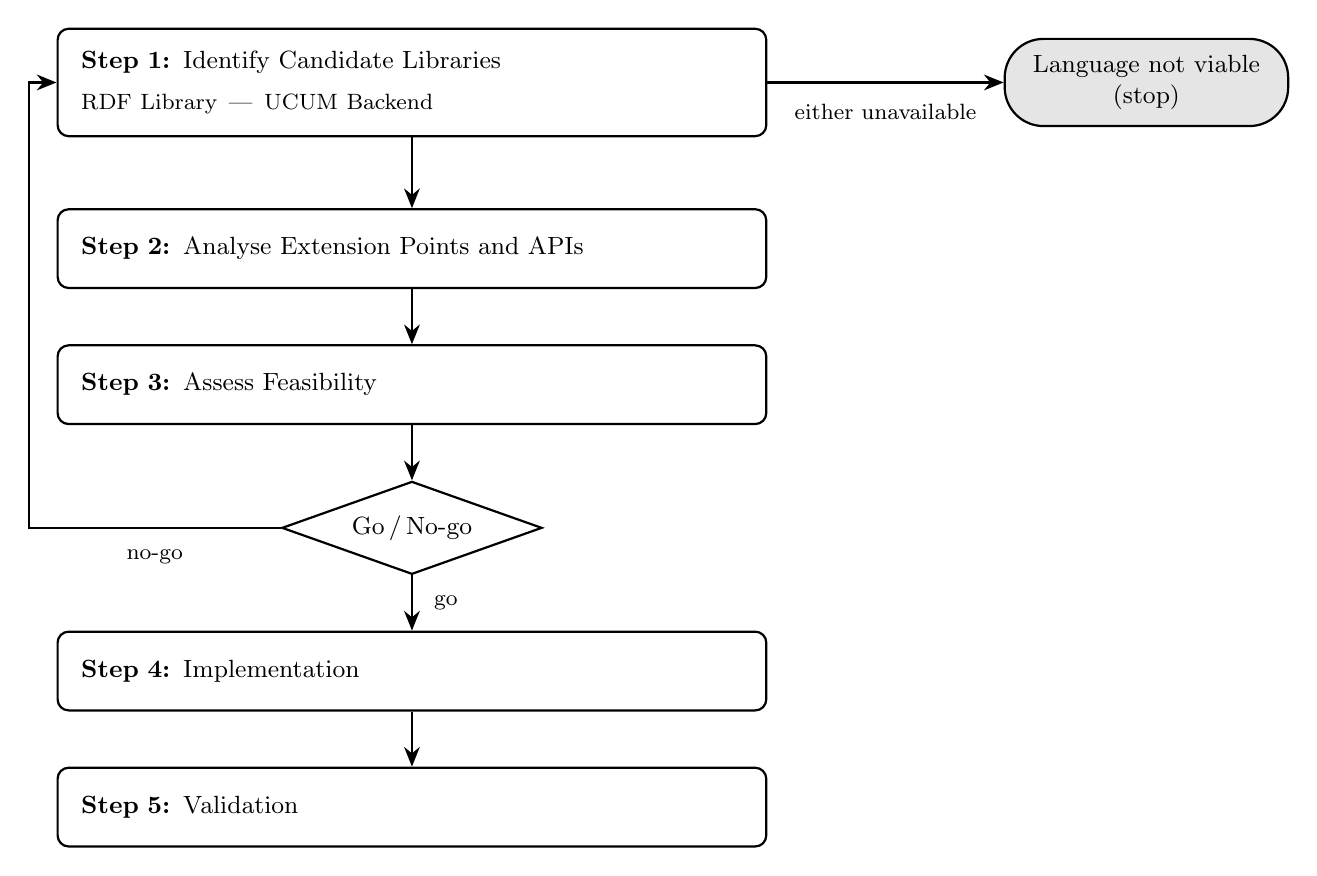
\begin{tikzpicture}[
    stepbox/.style={
        rectangle, draw, thick,
        rounded corners=4pt,
        minimum width=9.0cm,
        minimum height=1.0cm,
        text width=8.4cm,
        align=left,
        inner sep=8pt,
        font=\small
    },
    decnode/.style={
        diamond, draw, thick,
        minimum width=2.8cm,
        minimum height=0.9cm,
        align=center,
        font=\small,
        aspect=2.8
    },
    haltnode/.style={
        rectangle, draw, thick,
        rounded corners=14pt,
        fill=gray!20,
        minimum width=3.6cm,
        minimum height=0.9cm,
        align=center,
        inner sep=6pt,
        font=\small
    },
    arr/.style={-{Stealth[length=2.5mm,width=2mm]}, thick},
    lbl/.style={font=\footnotesize},
]

\node[stepbox] (s1) {%
    \textbf{Step 1:} Identify Candidate Libraries\\[4pt]%
    {\footnotesize RDF Library\enspace|\enspace UCUM Backend}%
};

\node[haltnode, right=3.0cm of s1] (stop) {Language not viable\\(stop)};

\node[stepbox, below=0.9cm of s1] (s2) {\textbf{Step 2:} Analyse Extension Points and APIs};
\node[stepbox, below=0.7cm of s2]  (s3) {\textbf{Step 3:} Assess Feasibility};
\node[decnode,  below=0.7cm of s3]  (gng) {Go\,/\,No-go};
\node[stepbox, below=0.7cm of gng] (s4) {\textbf{Step 4:} Implementation};
\node[stepbox, below=0.7cm of s4]  (s5) {\textbf{Step 5:} Validation};

% main flow
\draw[arr] (s1) -- (s2);
\draw[arr] (s2) -- (s3);
\draw[arr] (s3) -- (gng);
\draw[arr] (gng.south) -- node[lbl, right=1.5mm] {go} (s4.north);
\draw[arr] (s4) -- (s5);

% exit branch
\draw[arr] (s1.east) -- node[lbl, below=1.5mm] {either unavailable} (stop.west);

% no-go loop back
\draw[arr] (gng.west) -- node[lbl, below=1.5mm] {no-go} ++(-3.2,0) |- (s1.west);

\end{tikzpicture}
\caption{Five-step procedure with exit at Step~1 and go/no-go branch after Assess Feasibility}
\label{fig:five-step-procedure}
\end{figure}

\section{Identify Candidate Libraries}

The goal of this step is to identify two separate things: an RDF library to host the implementation, and a UCUM backend to handle unit parsing and arithmetic. The two searches are independent and proceed in parallel.

For the RDF library, the implementer must list the libraries available in the target language and subject each to a surface check covering three properties. The first is active maintenance, which is the floor rather than the whole of it: the library's age, contributor base, and breadth of adoption count alongside it, and a library may lack a major feature and still be the natural host if the community has settled on it. The second is SPARQL coverage; a library without a SPARQL engine is not discarded outright, but its available query mechanisms must be documented, because the operator obligations may still be deliverable in reframed form. The third is the presence of a custom datatype mechanism; without it, the registration obligation cannot be met.

For the UCUM backend, the implementer must identify libraries that can parse UCUM codes, convert between units, and perform arithmetic. Since UCUM-native libraries are scarce in most languages, the search must also include general unit-arithmetic libraries; these cannot serve alone but can pair with a UCUM-native parser. When a combination is chosen, the implementer must record which library handles which responsibility, because that boundary shapes the design of the internal quantity representation; two of the four implementations required this arrangement.

The step can produce a null result on either side. If no RDF library with a custom datatype mechanism exists for the target language, or no library or pairing can parse UCUM expressions and perform arithmetic at runtime, the shortlist on that side is empty. An empty shortlist on either side means implementation is not possible and the procedure stops.

The output is a shortlist of each kind, ordered by suitability, with the reason for every elimination recorded. The ordering matters because a no-go at the feasibility step returns to the next candidate on the shortlist rather than restarting the search.

\section{Analyze Extension Points and APIs}

The goal of this step is to read the internals of both shortlisted libraries and establish how each obligation of the specification maps onto what they actually expose.

For the RDF library, the analysis covers three areas. The first is datatype registration: how the library associates a datatype IRI with a custom type, what happens at parse time when a literal carrying that IRI is encountered, whether the association can be made from outside the core, and how the extension becomes active. The second is SPARQL operator evaluation: whether each evaluation point for equality, comparison, and arithmetic is exposed for extension or hardcoded, and when hardcoded, whether the host language permits runtime intervention from outside the library; the answer determines whether a workaround is available or the obligation requires a fork. The third area is the path from SPARQL constructs to those evaluation points: whether FILTER and BIND share the same machinery as ORDER BY and the aggregates SUM and AVG, or reach separate handlers, since the answers determine whether one hook covers everything or several are needed. Finally, the implementer must check whether the library provides a function registry invocable by IRI from inside a query; the sameDimension obligation depends on it.

For the UCUM backend, the analysis covers four areas. The first is the parsing API: what it accepts and returns. The second is arithmetic: whether the backend converts between units, tracks dimensions through operations, and signals incommensurable quantities. The third is the numeric type; a floating-point backend sets a precision ceiling no outer layer can raise. The fourth is coverage: whether all UCUM codes are supported or gaps exist.

The two cases examined here show why the analysis cannot stop at the library level. In Java, adjacent operators in the same engine received opposite answers; in Python, the operator module was reachable but ordering and aggregation held their own captured references, making an intervention appear complete while leaving those paths untouched.

The output of this step is a map from each obligation to the mechanism, if any, through which the library can satisfy it, together with the backend's capabilities and known gaps. This map is the sole input of the feasibility assessment that follows.

\section{Assess Feasibility}

The goal of this step is to decide, before any code is written, whether the candidate pair can satisfy the specification and to record how. The assessment runs through the obligations of Section 3.4 one by one.
One constraint frames the whole assessment: the implementation must be delivered as a standalone extension, ranking above every individual obligation. A fork produces a modified distribution users must run in place of the library they depend on and carry forward against every upstream release; Section 1 identified this as the shortcoming of the original Jena-ucum implementation. An obligation requiring a fork is recorded as not achievable.


For each obligation the assessment must reach one of three outcomes: satisfiable through a public API, satisfiable through a workaround, or not achievable without a fork. To reach the outcome, the implementer asks whether an extension point exists; if so, whether it is a documented public API or internals the library never promised to keep; and if not, whether the host language offers an alternative mechanism. The distinction matters because the cases age differently: a public API obligation survives upgrades, while a workaround must be re-verified at every upgrade and its interception points documented at the moment of choice.

The Python implementation shows the middle case. Comparison and arithmetic were not reachable through any public API: the engine validates operands against a fixed set of numeric types. The host language, however, permits replacing function references at runtime, so both were recorded as workarounds requiring re-verification at each library release.

When an obligation is not achievable, the implementer must either reframe it, delivering the same capability through a different interface, or return to Step 1 for the next candidate from the shortlist. The choice rests on three considerations: the centrality of the lost obligation, the availability of a viable shortlist alternative, and the library's weight in its ecosystem. A reframing must document what it achieves and gives up against the original wording; it is a documented deviation, not a fulfilment, and that record is what keeps the conformance claim honest.

The JavaScript implementation shows how ecosystem weight settles the choice. The library carries only a minimal query layer, placing the SPARQL operator obligations out of reach, yet it remains the library its community uses. 

The output of this step is a feasibility record stating, for each obligation, the case it falls under, the mechanism to be used, and any reframing adopted, together with the overall decision.


\section{Implementation}

The goal of this step is to turn the feasibility record into a working extension. The work follows a fixed order because each part depends on the one before it: the quantity representation first, registration second, the SPARQL hooks third, and the custom function fourth.

The implementer must begin with a class that wraps the UCUM backend and exposes every operation the value space requires: parsing a lexical form and writing one back, equality, comparison, arithmetic, unit conversion, and the dimension test. All backend access must pass through this class, keeping the rest of the extension independent of its API. The class must realise the value space defined in Section 3.4: two quantities in different units of the same dimension that denote the same value must compare as equal. Where the first step selected a pairing rather than a single backend, the division of labour recorded there becomes the internal structure of this class; the parser produces what the arithmetic library consumes.
With the representation in place, the implementer must register cdt:ucum and cdt:ucumunit through the extension point recorded in the feasibility record, after which the library parses a CDT literal into a typed object rather than an opaque string. 

The SPARQL hooks come next. The implementer must intercept equality, comparison, and arithmetic through the mechanisms recorded per obligation, and every handler must follow the same pattern: check whether the operands are CDT literals, evaluate them through the representation if they are, and pass the call to the original behaviour unchanged if they are not. The fallback matters as much as the interception, because the extension must leave the engine's treatment of every other datatype exactly as it found it. Ill-typed literals must be caught before any value operation and routed into the engine's error path, so that the affected solution is excluded, as Section 2.3 described, rather than the whole query failing. The map from the analysis step states how many interception points this takes and where none is needed. In two implementations, registration alone already delivered SPARQL equality. In the Python case, the interception reached twenty-five points across four modules.

The custom function completes the operator work. The implementer must register cdt:sameDimension through the function registry recorded in the analysis. The function extracts two quantities, asks the backend whether their dimensions match, and returns a boolean.

Implementation surfaces five cases that the analysis cannot show in advance and that must be expected in any new implementation. The first is units the backend cannot parse, with the special units of Section 3.3 first among them. The second is comparison across dimensions inside ORDER BY; the query must never abort on such data, and since SPARQL leaves this ordering undefined, any deterministic grouping or fallback is conformant. The third is unit preservation in SUM, AVG, MIN and MAX, where the engine's own accumulators work on bare numbers and would return a result stripped of its unit. The fourth is precision at the numeric extremes, where the backend's internal number type sets a ceiling no outer layer can lift. The fifth is the dimensionless case: a bare number must be read as a quantity with the unit one. Each case must be handled explicitly and the chosen behaviour written down, because several will return in the next step as expected failures.

The output of this step is the working extension together with the record of edge cases and the behaviour chosen for each. That record joins the feasibility record as input to the validation step.

\section{Validation}

The goal of this step is to verify that the extension satisfies each obligation it claims and to document what it does not. The output is not a count of passing tests but an account of conformance in which every claim is backed by a test and every limitation is visible.

The implementer must first test each obligation of Section 3.4. For lexical parsing, both valid and invalid inputs must be tested: a valid UCUM expression must parse to the correct value, and an invalid one must be rejected as ill-typed. Value equality is tested across units of the same dimension, including derived units and the dimensionless case. Comparison is tested within one dimension and across dimensions, where the error required by the specification must be raised. Arithmetic is tested over its full type coverage, including scalar operands on both sides of the operator. The dimension test is checked with compatible and incompatible pairs.
Each obligation must be tested at the level at which the feasibility record claims it. An obligation claimed at the query level requires tests that submit a query and inspect the results: a correct method the engine never calls passes every direct test and still fails the claim. Where an obligation was reframed, the tests target the reframed interface; no test may suggest the original form is available. The Python implementation tests at both levels: the quantity class directly, and the operators, ordering, and aggregates through queries. The Java implementation exercises equality through its interface but submits no query, so the query-level behaviour rests on the engine's documented routing rather than a test of this extension. The difference between these two positions is exactly what this step must make visible.

The implementer must then test the edge cases recorded during implementation. A query over data containing an ill-typed literal must complete, with the affected solutions excluded. Ordering over mixed dimensions must complete and follow the behaviour chosen for it. The aggregates must preserve units where the implementation claims they do. Precision is tested at scales far above and below the range of ordinary values, where the backend's numeric ceiling either holds or breaks. A literal written out and parsed back must keep its value. Activating the extension more than once must change nothing.

What the feasibility record marked as not achievable must now appear as expected failures. For each limitation, the implementer must write the test it causes to fail, mark it as expected, and attach the reason stating whether the cause is an inherited dependency limit or a gap in the extension itself; the two call for different responses from anyone who later builds on the work. A limitation carried this way is checked on every run and announces itself when a dependency upgrade removes it; one left out of the suite stays silent. The same two families recur across all four implementations: the special units of Section 3.3, whose conversion falls outside the algebra every backend implements, and precision loss where a backend computes in a bounded numeric type. A new implementation should expect to document both.

The output is the test suite together with the conformance account it expresses: the obligations met, the level at which each is met, the reframings, and the expected failures with their reasons. That account makes the extension's claims checkable by someone who did not build it, and is the form in which the four implementations are reported in Section 6.
\chapter{Implementations and Findings}

This chapter reports the four implementations that validate the methodology of Chapter 5. It is organised by the five steps of that methodology rather than by library. Each section takes one step and reports how all four implementations met it, so that the section reads as a test of that step across four environments. Sections 6.1 to 6.5 follow the five steps in order. Section 6.6 collects the findings that recur across the cases.

The four implementations appear in the same fixed order throughout the chapter: Apache Jena in Java, rdflib.js in TypeScript, dotNetRDF in C\#, and RDFLib in Python. Table 3 sets them side by side from host library to standout limitation.

\begin{table}[h]
\centering
\caption{The four implementations from host to outcome. Repositories are at \texttt{github.com/Irfan-Ullah-cs/}.}
\label{tab:implementations-overview}
\small
\renewcommand{\arraystretch}{1.3}
\begin{tabularx}{\textwidth}{@{}>{\raggedright\arraybackslash}p{3.2cm} *{4}{>{\raggedright\arraybackslash}X}@{}}
\toprule
 & Apache Jena (Java) & rdflib.js (TypeScript) & dotNetRDF (C\#) & RDFLib (Python) \\
\midrule
Host library       & Jena 6.0.0            & rdflib.js   & dotNetRDF      & RDFLib 7.6.0 \\
UCUM backend       & systems-ucum + Indriya & ucum-lhc   & Fhir.Metrics   & ucumvert + Pint \\
SPARQL engine      & full                  & none        & full           & full \\
Operator delivery  & equality in query, rest reframed onto Java API & reframed onto store API & on the query surface & on the query surface \\
Numeric precision  & fixed-precision decimal & double precision & decimal, \textasciitilde{}28 digits & arbitrary-precision decimal \\
Tests              & 163                   & 157         & 251            & 253 \\
Repository         & \href{https://github.com/Irfan-Ullah-cs/jena-ucum}{jena-ucum} & \href{https://github.com/Irfan-Ullah-cs/rdflib.js-ucum}{rdflib.js-ucum} & \href{https://github.com/Irfan-Ullah-cs/dotnetrdf-ucum}{dotnetrdf-ucum} & \href{https://github.com/Irfan-Ullah-cs/rdflib-ucum}{rdflib-ucum} \\
\bottomrule
\end{tabularx}
\renewcommand{\arraystretch}{1}
\end{table}

Each section reports the information that determined a decision, named a mechanism, or produced a limitation. The full detail for each implementation is in the public repository.


\section{Identify Candidate Libraries}

This step looks for two things in each language: an RDF library to host the implementation and a UCUM backend to parse and compute. A short survey of each ecosystem is usually enough to see the landscape. RDF libraries can be compared on a handful of ordinary signals, none decisive alone: how long the library has existed, how widely it is adopted, how many people contribute to it, and how complete its feature set is. Completeness sits among these signals rather than above them. A library can lack a major feature and still be the natural choice, because a community has settled on it and built real systems on top of it. Adoption of that kind is its own kind of evidence. On the backend side the field in every language is narrow, and the property that matters most is whether a library can take an arbitrary UCUM expression at runtime rather than a fixed vocabulary set in advance.

For three of the four languages the survey points to one library without much contest. In Python, RDFLib has been the general-purpose RDF library of the ecosystem for over two decades, with the broadest contributor base of the hosts considered here and a full SPARQL 1.1 engine written in Python. In JavaScript, rdflib.js holds a long-established place among Linked Data applications; Section 4.2 records that it is a read-write Linked Data toolkit rather than a query engine, yet its adoption and its role in the community are what recommend it, the missing engine not withstanding. In C\#, dotNetRDF has been maintained since 2009 and ships the established in-process SPARQL 1.1 engine of the .NET world. 

Java is the exception, and deliberately so. The implementation accompanying the CDT specification was a fork of Apache Jena built against version 3, with the datatype behaviour hardcoded into the modified distribution. Jena was kept for this thesis to ask a specific question: how much of what the fork achieved from the inside can be recovered from the outside, as a standalone extension that leaves the library untouched. Carrying the work forward also meant moving from Jena 3 to the current 6.0.0. Eclipse RDF4J is the other mature Java host and nothing here counts against it; Jena was the platform the prior work sat on, and continuing that work is the point of the case.

The backends were chosen on the same mixture of capability and standing. In Java the work inherited the JSR-385 pairing already used in the fork, with systems-ucum supplying the UCUM grammar and unit definitions and Indriya the conversion and arithmetic. In JavaScript, ucum-lhc comes from the Lister Hill Center of the US National Library of Medicine and covers validation, conversion, and decomposition to SI base units on its own. In C\#, Fhir.Metrics, developed by Firely for the FHIR standard, loads the official UCUM definition file at runtime and parses expressions from the string. Python takes the same paired shape as Java. No single Python library does both: ucumvert is the only native UCUM parser, young but generated directly from the official UCUM definition file, and it computes through Pint, the established unit-arithmetic library of the ecosystem. So two of the four languages pair a UCUM-specific parser with a general arithmetic engine, ucumvert with Pint and systems-ucum with Indriya, while C\# and JavaScript each have a single library that does both.

What this step cannot settle is how far each host can be reached from outside. That is the question the next section takes up, and in Java it is the whole point of the case.


\section{Analyze Extension Points and APIs}

This step reads the internals of each host and each backend to learn what is reachable and how. The question divides three ways: how the library turns a typed literal into a value at parse time, where and whether it lets an extension reach the SPARQL operators, and what the backend offers for parsing and arithmetic. The answers vary more between the four hosts than any other step in the chapter, and that variance is the finding.

Datatype registration is the one area where every host offered a usable path, though of different kinds. RDFLib exposes a documented function, bind, that ties a datatype IRI to a value class and a constructor, after which the library calls the constructor on the lexical form at parse time and stores the result. Jena exposes a comparable public registry, TypeMapper, and calls the registered datatype's parse method when it reads a matching literal, marking the literal ill-typed if the parse throws. dotNetRDF has no single registration call. Recognition is achieved instead by subclassing the graph so that literal creation returns a quantity node for the cdt:ucum IRI, and by adding that IRI to the engine's list of recognized types so the comparison machinery treats it as a value rather than an opaque string. rdflib.js offers nothing here at all: its literal constructor performs no dispatch on the datatype IRI and calls no registered code, so a cdt:ucum literal is stored exactly like any other typed string. The consequence for rdflib.js is that recognition has to live inside the extension and be applied wherever literals enter it, the situation Chapter 5 describes for a host with no registration mechanism.

The SPARQL operators are where the hosts diverge most, and Jena is the clearest case because its engine treats its own operators inconsistently. Equality is delegated. When ARQ evaluates the equality operator on two typed literals it routes the call, through its literal layer, to the registered datatype's own equality method. Implementing that method is all native SPARQL equality requires, with no interception of any kind. Comparison and arithmetic are not delegated. The less-than and greater-than operators, the four arithmetic operators, the ORDER BY comparator, and the SUM and AVG accumulators all evaluate inside engine code that consults no registry and calls no method on the datatype; an unrecognized type raises an internal error. There is no interface to implement and no registry to populate for these, and compiled Java offers no stable way to intervene from outside. The split is therefore imposed by the engine: one obligation reachable through a clean public method, the rest reachable only by forking.

The other three hosts each sit at a different point. dotNetRDF is the most accommodating: arithmetic operators can be added through a public operator registry, equality follows from adding the datatype to the recognized-types list, the node comparer used in filters is a public settable property, and custom functions have a public factory. Only one operator path, the ORDER BY comparer, has no public setter, and it is reachable through a single reflective access to a private field, the one non-public point in the whole extension. RDFLib exposes none of these as extension points, but Python permits replacing functions at runtime, so the operators are reachable by patching, and the patching has to reach further than it first appears. The operator functions live in one module, but the parser holds its own references to them captured when it loads, and ordering and the aggregates hold further references of their own in separate modules. A change to the operator module alone would leave those paths running the original code while looking complete. rdflib.js has almost no SPARQL surface to reach: its query layer evaluates only basic patterns and equality filters, the three comparison operators all collapse to equality, and ordering, binding, and aggregates are absent. There is no function registry. What it does expose is a native query API on the store, and one method on it is the funnel the others pass through, which is the single point the extension can use.

Two structural questions from Chapter 5 resolved consistently across the hosts that have the machinery at all. Where filters and value-binding expressions exist, they share one evaluation path, so a single interception covers both. Ordering and the aggregates do not share that path; they run through separate code and must be reached separately. Jena, dotNetRDF, and RDFLib each confirm this division in their own terms, and it is the reason Chapter 5 warns against assuming one hook suffices.

The backends were read for three things: what their parser accepts and returns, whether they perform dimensional arithmetic with an error on incommensurable operands, and what numeric type they compute in. All four parse an arbitrary UCUM expression and perform dimensional arithmetic. Three of the four signal incompatible dimensions correctly, by an exception or by a failure status the extension turns into one. The fourth does not. The C\# backend treats some distinct dimensions as the same, newton and pascal among them, so an addition that should be rejected is accepted. Section 6.3 returns to this. The numeric type is where they part company, and the difference sets a ceiling no outer layer can lift. The Python backend can be configured to compute in arbitrary-precision decimal, and once a hidden fallback to floating point in the parser's transformer is corrected, it does so throughout. The C\# backend computes in the platform decimal type, roughly twenty-eight significant digits, with an overflow above that range, and like the Java backend it rounds non-terminating conversion factors to that fixed precision. The JavaScript backend computes in double-precision floating point only, as defined by IEEE 754 \cite{ieee2019_754}, with no higher-precision mode, so any precision beyond a double is lost before arithmetic begins. The Java backend keeps exact precision for integer-ratio conversions but rounds non-terminating conversion factors to a fixed decimal precision, a limitation the validation section returns to. Each backend's coverage gaps were also recorded here, and they converge on the special units of Section 3.3, which the next sections report where they surface as outcomes.

This step produced, for each host, a map from every obligation to the mechanism that can satisfy it or the absence of one. Those maps are what the feasibility assessment in the next section reasons over.

\section{Assess Feasibility}

Feasibility reads over the two maps from the previous section. One records how each host exposes the operators and the registration mechanism. The other records what each backend offers for parsing and arithmetic. The obligations of the specification guide this reading, but they do not decide it on their own. A library can be the right host even when it cannot meet every obligation, because a community has already settled on it and builds real work on top of it. That standing is part of the evidence, alongside the maps. All four candidates returned a go. What differed was what the go required.

The backend side carries one gate above the others. The backend must take an arbitrary UCUM expression at runtime and perform dimensional arithmetic on it. This gate already did work in the first step, where it removed the libraries that fix their unit vocabulary at compile time. The four chosen backends all pass it. They part company on the numeric type they compute in, and the feasibility step accepts that ceiling because no outer layer can raise it. The Python backend computes in arbitrary-precision decimal, the highest of the four. The JavaScript backend computes in double precision, the lowest.

For Jena, the go required accepting that two obligations cannot be reached from outside the library. Registration, equality, and the sameDimension function are met through public APIs. Comparison and arithmetic are not. The engine evaluates them in code that consults no registry, and compiled Java offers no way in from outside without a fork. This does not make the host unusable. Jena still parses a document carrying the datatype, still recognizes the literals, and still answers the simple queries that rest on parsing and equality.

For rdflib.js, the go rests on the same kind of reasoning at a wider scale. The library has no registration mechanism and a query layer that reduces the three comparison operators to equality, so most of the operator obligations cannot be reached inside a query at all. By an obligation count alone it would look like a poor candidate. It is not, because it holds a long-established place among Linked Data applications and is the library that community reaches for. The obligations it can meet are reframed onto its native store API, the one surface the extension can intercept, and the rest are delivered through an explicit operations layer. The backend passes the runtime gate but computes in double precision, so the go is recorded together with that ceiling.

For dotNetRDF, every obligation is reachable on the query surface, through public registries and one reflective access for the ordering comparer. One backend limitation is recorded here rather than left for later. The Fhir.Metrics dimensional check compares unit axes without their exponents. It therefore reports some distinct dimensions as the same, newton and pascal among them. The extension checks that result before adding, so an addition the specification requires to fail does not fail. This is a defect in the backend, not in the extension, and the go is taken with it documented.

For RDFLib, the go is the most complete of the four. Every obligation is met. Three are met through public APIs. The other two are met by replacing the operator functions at runtime, and those replacements are reversible and produce results the specification accepts. The backend computes in arbitrary-precision decimal once a single fallback in the parser is corrected.

All four are a go. Two reached it with every obligation on the query surface, dotNetRDF and RDFLib. Two reached it by moving obligations off that surface, Jena and rdflib.js. The rule against forking the host is what separates the two pairs. Underneath all four sits the same idea: the obligations shape the decision, but a host is chosen because it is useful and used, and a partial fit on a library a community trusts is worth more than a full fit on one nobody runs.


\section{Implementation}

This step turns the feasibility record into a working extension. The four implementations built in the same fixed order: the quantity representation first, registration second, the SPARQL hooks third, the custom function fourth, and the edge cases last. Each part depends on the one before it, because registration produces objects of the representation and the hooks evaluate those objects.

The representation is a single class that wraps the backend and exposes every operation the value space needs: parsing a lexical form and writing one back, equality, comparison, arithmetic, conversion, and the dimension test. All backend access passes through it, so the rest of the extension stays independent of the backend's API. In the C\# implementation one source file is the only place that touches Fhir.Metrics. Where the first step chose a pairing rather than a single backend, that division becomes the internal structure of the class: in Python and Java the parser produces what the arithmetic library consumes. The class realises the value space of Section 3.4, so two quantities in different units of the same dimension that denote the same value compare as equal.

Registration ties cdt:ucum and cdt:ucumunit to the representation through the mechanism the feasibility record named, after which the host parses a CDT literal into a typed object rather than an opaque string. Two matters are settled here. Registering twice must be harmless, because a host application cannot be stopped from doing it. And where the library attaches no behaviour to a datatype IRI, recognition has to live inside the extension and be applied wherever literals enter it. rdflib.js works this way, carrying its own recognition into every operation.

The SPARQL hooks follow one pattern in every implementation. A handler checks whether its operands are CDT literals. If they are, it evaluates them through the representation. If they are not, it hands the call back to the original behaviour unchanged, so the engine's treatment of every other datatype is left exactly as it was. Ill-typed literals are caught before any value operation and routed into the engine's error path, so the affected solution is dropped rather than the whole query failing. How many interception points this takes is what most separates the four. In two of them, Jena and dotNetRDF, registration alone already delivered SPARQL equality, because the engine routes equality of typed literals through the registered datatype. Python sits at the other end. The operator functions, the ordering routine, and the aggregate accumulators each held their own references, and the interception reached twenty-five points across four modules before the engine behaved consistently.

The custom function cdt:sameDimension was the simplest obligation wherever a registry existed. It extracts two quantities, asks the backend whether their dimensions match, and returns a boolean.

Implementation surfaces cases the analysis cannot show in advance, and the same five recur. Units the backend cannot parse, the special units of Section 3.3 first among them. Comparison across dimensions inside ORDER BY, which must never abort the query. Unit preservation in SUM and AVG, whose accumulators work on bare numbers and would otherwise strip the unit. Precision at the numeric extremes, where the backend's number type sets the ceiling. And the dimensionless case, where a bare number must be read as a quantity with the unit one, which more than one backend needed a dedicated branch to do. Each was handled explicitly and the chosen behaviour written down, because several return in the next step as expected failures.


\section{Validation}

This step verifies that each implementation satisfies the obligations it claims and documents what it does not. It does not let each implementation grade itself against its own tests. Before any library was tested, a single reference set of behavioral requirements was drawn up, setting out what a complete implementation should be tested for, independent of any one language. Each of the four suites is then read against that same reference, and every requirement receives a status: covered, covered but behaving differently in a documented way, not applicable to the language, or absent. Reading all four against one checklist is what lets them be compared on equal terms. The result that matters is not a count of passing tests. It is an account of conformance in which every claim is backed by a test and every limitation is visible.

The four suites differ in size, and the sizes are worth reading, though not as a score, since a larger suite is not a more conformant one. RDFLib has the most at 253 tests, no fail tests. dotNetRDF has 251, of which thirty-eight are left failing; the validation step below records which cases take which form. Jena has 163 and rdflib.js 157. What the totals hide, the distribution shows, because the shape of each suite tracks where its operators live. In RDFLib the operators run through the engine, and the query file alone holds sixty-nine tests. In rdflib.js the same obligations are reframed onto the store API, and the query file holds nine, with the weight moved to parsing and arithmetic tested on the quantity class directly. Jena has no query-level test file at all, and its largest class, sixty-seven tests, exercises the Java operations API that comparison and arithmetic were reframed onto. The reframings of Section 6.3 are visible in the counts.

Each obligation is tested at the level at which the feasibility record claims it. This distinction does real work. An obligation claimed at the query level needs a test that submits a query to the engine and reads the result, because a correct method the engine never calls passes every direct test and still fails the claim. The Python implementation tests at both levels: the quantity class on its own, and then the operators, ordering, and aggregates again through queries the engine runs. The Java implementation exercises its equality mechanism through the datatype interface but submits no query, so its query-level equality rests on Jena's documented routing rather than on a test of the extension. Making that difference visible is part of the step. Arithmetic is tested across its full type coverage, and two of the four were incomplete at the same point.

The edge cases recorded during implementation are tested next. A query over data that contains an ill-typed literal must complete with the affected solutions excluded, not abort. Ordering over mixed dimensions must complete and follow the behaviour chosen for it. The aggregates must preserve units where the implementation claims they do. A literal written out and parsed back must keep its value. Activating the extension more than once must change nothing.

What the feasibility record marked as not achievable appears here as expected failures, each with the test that fails and the reason attached, stating whether the cause is a limit inherited from a dependency or a gap in the extension. Two families recur across all four. The special units of Section 3.3, whose conversion falls outside the algebra every backend implements, and precision loss where a backend computes in a bounded numeric type. The form these take differs with the backend. Where a backend's lower precision is itself the accepted behaviour, that boundary becomes a passing test that documents the loss: rdflib.js records a value beyond double range collapsing to infinity and the sixteenth-digit case collapsing to one float. dotNetRDF records all limitations as failing tests. Its decimal backend overflows above roughly twenty-eight significant digits and rounds non-terminating conversion factors, both recorded as failing tests; the latter is why a cross-unit equality such as 3.6 km/h against 1 m/s does not hold. The Celsius offset conversion and the Fhir.Metrics dimensional defect that reports newton and pascal as one dimension are also left as failing tests with the cause attached. In all, the suite leaves thirty-eight tests failing.

The output of the step is the test suite together with the conformance account it expresses: the obligations met, the level at which each is met, the reframings, and the expected failures with their causes. That account is what lets someone who did not build the extension check its claims, and because all four are written against one reference, read the four side by side.


\section{Findings Across the Cases}

The clearest finding of the chapter is that the same obligation landed differently in each host, and for one reason: how far an extension could reach into the host from outside. That reach is set by two things. The first is the host's architecture, whether it exposes its operators through a public point or evaluates them in code an extension cannot enter. The second is the host language. A dynamic language lets an extension replace functions at runtime, which is how the Python operators were reached at twenty-five points without altering the library. A compiled language offers no such entry, so the extension is held to whatever public points exist, and where there are none, as with Jena's comparison and arithmetic, the only ways left are to fork or to reframe. The variance across the four is not noise around a single result. It is the result, and a go or no-go follows from the host's architecture and its standing rather than from counting obligations met.

The rule against forking sorts the four into three positions. RDFLib and dotNetRDF keep every obligation on the SPARQL query surface. Jena has a full SPARQL engine but its comparison and arithmetic operators are evaluated inside engine code that exposes no public extension point; those obligations are reframed onto an explicit Java API while equality remains on the query surface. rdflib.js has no complete SPARQL engine. All four stay worth implementing because they are the libraries their communities use. A partial fit on a trusted host is worth more than a complete fit on one no one runs.

Table 3 sets the four implementations side by side, from the host each ran on to the limitation each carries. All four returned a go; the table shows what the go required of each.

Where the hosts diverge, the backends converge. The gaps that recur are not host-specific but backend-specific, and the same two appear whatever the language. The special units of Section 3.3, whose conversion falls outside the algebra every backend implements, and precision loss wherever a backend computes in a bounded numeric type. The numeric ceiling is the sharpest case of the second. It is set by the backend, not the host, ranges from arbitrary-precision decimal in Python to double precision in JavaScript, and no layer above the backend can raise it.
\chapter{Conclusions}

This thesis set out to determine whether implementing cdt:ucum in an RDF library could be turned from a one-off effort into a general procedure. It produced a five-step methodology and validated it through four standalone implementations, in Java, TypeScript, C\#, and Python. Each leaves its host library unmodified, and each is tested against a single reference checklist so that the four can be read side by side. The procedure assumes no particular language and no particular library architecture, and the four cases show it holding across environments that differ in both.

The four cases also produced a finding that none of them shows alone. The obligations of the specification are fixed, but how far an extension can reach into a host from the outside is not, and that reach is what decides how each obligation gets met. It is set by two things: whether the host exposes its operators through a public point or evaluates them in code an extension cannot enter, and whether the host language permits intervention at runtime. The same specification was therefore satisfied through different mechanisms in each of the four hosts, and which mechanism applied followed from these two properties rather than from the obligations themselves.

\textbf{Future Work: } The clearest continuation is to apply the methodology to RDF libraries it has not yet met. RDF4J is the other major Java library; running the procedure there holds the language fixed and changes only the host architecture, isolating how much of the outcome that architecture alone decides. Sophia and rdf4cpp carry the procedure into Rust and C++, two languages absent from the four cases, where the runtime intervention that the Python implementation relied on has no obvious equivalent and the question of what reach remains is open. Each new host added this way sharpens the same map the methodology exists to draw.
\printbibliography[title={References}]
\end{document}